\documentclass[12pt]{article}
\usepackage[czech]{babel}
\usepackage[utf8]{inputenc}
\usepackage[plainpages=false,pdfpagelabels,unicode]{hyperref}
\usepackage[pdftex]{graphicx}
\usepackage[margin=2cm, includefoot]{geometry}

\begin{document}

\title{Praktikum z fyziky plazmatu \\
Měření prvního Townsendova koeficientu}
\author{Pavel Ondračka}
\maketitle

\section{Úvod}
Svazek elektronů, vznikajících fotoemisí z katody vlivem ultrafialového záření urychlujeme homogenním elektrickým polem. Elektrony při průchodu plynem způsobují ionizaci a nakonec dopadají na anodu. Pro proud mezi dvěma elektrodami platí $I=I_0 \mathrm{e}^{\alpha x}$.
Koeficient $\alpha$ závisí na intenzitě elektrického pole a na tlaku (na $E$ závisí energie získaná na střední volné dráze, na tlaku pak samotná velikost střední volné dráhy).
V obecné případě lze tuto závislost psát ve formě $\frac{\alpha}{p} = A \mathrm{e}^{\frac{-B p}{E}}$,
kde $A$ a $B$ jsou konstanty.

\begin{figure}[htbp]
\begin{center}
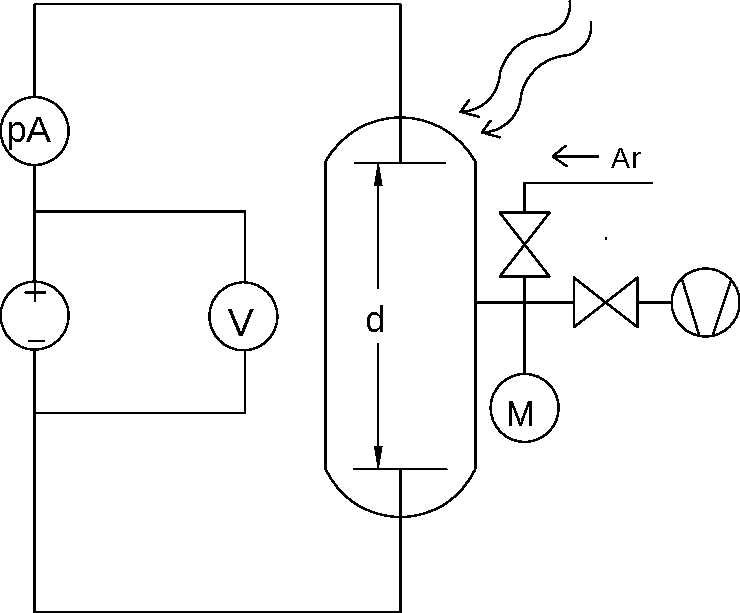
\includegraphics[width=10cm]{nakres.pdf}
\caption{Schéma aparatury, pA -- pikoampermetr, V -- voltmetr, M -- manometr}
\label{schema}
\end{center}
\end{figure}

\section{Měření}
\begin{boldmath}
\large{\bf{2.1\,\,\,Proveďte měření závislosti  $I=f(x)$  pro daný tlak plynu ve výbojce a pro pět hodnot intenzity elektrického pole ve výbojovém prostoru. Vyneste závislosti do grafu a stanovte z nich $\alpha$, $I_0$, $A$ a $B$.}}\\
\end{boldmath}


Měření bylo prováděno pro hodnoty el. pole 80\,V/cm, 100\,V/cm, 110\,V/cm, 120\,V/cm a 130\,V/cm. 
Hodnoty na pikoampérmetru během měření mírně oscilovaly, proto byl pro každou vzdálenost elektrod proud naměřen čtyřikrát a 
vypočítán průměr. Převrácený čtverec směrodatné odchylky byl pak použit jako váha pro fitování.

\begin{table}[htbp]
\begin{center}
\begin{tabular}{|c|c|c|c|c|c|c|}
\hline
$x$[mm] & $I$[pA] & $\sigma_I$[pA] & $I_1$[pA] & $I_2$[pA] & $I_3$[pA] & $I_4$ [pA] \\ \hline
20 & 186,55 & 1,77 & 186,7 & 188,3 & 184,1 & 187,1 \\ \hline
18 & 138,40 & 1,46 & 139,4 & 137,1 & 139,9 & 137,2 \\ \hline
16 & 102,08 & 1,52 & 103,4 & 99,9 & 102,3 & 102,7 \\ \hline
14 & 78,17 & 1,28 & 80 & 77 & 77,77 & 77,9 \\ \hline
12 & 57,70 & 1,31 & 59,3 & 57,6 & 57,8 & 56,1 \\ \hline
10 & 42,38 & 0,30 & 42,7 & 42,3 & 42,5 & 42 \\ \hline
8 & 31,38 & 1,10 & 32,7 & 31,7 & 31 & 30,1 \\ \hline
6 & 21,85 & 0,70 & 21,1 & 22,4 & 22,5 & 21,4 \\ \hline
4 & 14,73 & 0,67 & 15,4 & 14,2 & 15,2 & 14,1 \\ \hline
2 & 10,45 & 1,16 & 10,6 & 11,5 & 10,9 & 8,8 \\ \hline
\end{tabular}
\caption{$E = 80\,\mathrm{V/cm}$}
\label{t80}
\end{center}
\end{table}

\begin{table}[htbp]
\begin{center}
\begin{tabular}{|c|c|c|c|c|c|}
\hline
$x$[mm] & $I$[pA] & $\sigma_I$[pA] & $I_1$[pA] & $I_2$[pA] & $I_3$[pA] \\ \hline
20 & 177,13 & 1,96 & 175,1 & 179 & 177,3 \\ \hline
18 & 123,20 & 0,79 & 122,6 & 124,1 & 122,9 \\ \hline
16 & 86,73 & 2,89 & 83,6 & 87,3 & 89,3 \\ \hline
14 & 59,13 & 0,68 & 58,6 & 58,9 & 59,9 \\ \hline
12 & 41,90 & 0,87 & 42,3 & 42,5 & 40,9 \\ \hline
10 & 28,47 & 0,67 & 28,3 & 27,9 & 29,2 \\ \hline
8 & 20,70 & 0,10 & 20,8 & 20,6 & 20,7 \\ \hline
6 & 14,47 & 0,47 & 15 & 14,3 & 14,1 \\ \hline
4 & 9,00 & 0,10 & 9,1 & 9 & 8,9 \\ \hline
2 & 5,00 & 0,92 & 6 & 4,8 & 4,2 \\ \hline
\end{tabular}
\caption{$E = 100\,\mathrm{V/cm}$}
\label{t100}
\end{center}
\end{table}

\begin{table}[htbp]
\begin{center}
\begin{tabular}{|c|c|c|c|c|c|c|}
\hline
$x$[mm] & $I$[pA] & $\sigma_I$[pA] & $I_1$[pA] & $I_2$[pA] & $I_3$[pA] & $I_4$ [pA] \\ \hline
20 & 166,35 & 2,81 & 168,8 & 162,5 & 168 & 166,1 \\ \hline
18 & 102,85 & 3,87 & 101,1 & 102,9 & 99,2 & 108,2 \\ \hline
16 & 64,20 & 1,12 & 65,4 & 64,9 & 63,1 & 63,4 \\ \hline
14 & 40,20 & 4,26 & 45,7 & 40,5 & 35,4 & 39,2 \\ \hline
12 & 25,05 & 2,63 & 28,9 & 23,7 & 23,1 & 24,5 \\ \hline
10 & 13,43 & 0,67 & 13 & 14,4 & 13 & 13,3 \\ \hline
8 & 7,10 & 1,14 & 6,7 & 7,7 & 8,3 & 5,7 \\ \hline
6 & 2,38 & 0,21 & 2,6 & 2,2 & 2,5 & 2,2 \\ \hline
4 & -0,75 & 0,73 & -0,9 & -1 & -1,4 & 0,3 \\ \hline
2 & -2,00 & 0,81 & -1,4 & -1,7 & -3,2 & -1,7 \\ \hline
\end{tabular}
\caption{$E = 110\,\mathrm{V/cm}$}
\label{t110}
\end{center}
\end{table}

\begin{table}[htbp]
\begin{center}
\begin{tabular}{|c|c|c|c|c|c|c|}
\hline
$x$[mm] & $I$[pA] & $\sigma_I$[pA] & $I_1$[pA] & $I_2$[pA] & $I_3$[pA] & $I_4$ [pA] \\ \hline
20 & 169,43 & 1,85 & 167,7 & 171,4 & 168 & 170,6 \\ \hline
18 & 104,08 & 1,82 & 106,5 & 104 & 102,1 & 103,7 \\ \hline
16 & 60,65 & 1,80 & 61,9 & 61,6 & 61,1 & 58 \\ \hline
14 & 37,60 & 0,67 & 38,3 & 37,8 & 37,6 & 36,7 \\ \hline
12 & 22,78 & 0,10 & 22,9 & 22,8 & 22,7 & 22,7 \\ \hline
10 & 12,48 & 0,45 & 13,1 & 12,5 & 12,2 & 12,1 \\ \hline
8 & 6,45 & 1,05 & 6,3 & 6,8 & 5,1 & 7,6 \\ \hline
6 & 2,78 & 0,71 & 3,4 & 2,5 & 1,9 & 3,3 \\ \hline
\end{tabular}
\caption{$E = 120\,\mathrm{V/cm}$}
\label{t120}
\end{center}
\end{table}


\begin{table}[htbp]
\begin{center}
\begin{tabular}{|c|c|c|c|c|c|c|}
\hline
$x$[mm] & $I$[pA] & $\sigma_I$[pA] & $I_1$[pA] & $I_2$[pA] & $I_3$[pA] & $I_4$ [pA] \\ \hline
18 & 172,73 & 1,81 & 173,8 & 171,9 & 170,6 & 174,6 \\ \hline
16 & 97,53 & 1,25 & 97,4 & 97,9 & 98,9 & 95,9 \\ \hline
14 & 56,40 & 0,83 & 56,4 & 55,3 & 56,6 & 57,3 \\ \hline
12 & 32,58 & 0,79 & 32,2 & 33,7 & 31,9 & 32,5 \\ \hline
10 & 17,48 & 0,36 & 18 & 17,4 & 17,2 & 17,3 \\ \hline
8 & 7,90 & 0,52 & 7,3 & 8,5 & 8,1 & 7,7 \\ \hline
6 & 2,90 & 0,29 & 3,2 & 3 & 2,5 & 2,9 \\ \hline
4 & 0,13 & 0,85 & 1,3 & -0,2 & 0,1 & -0,7 \\ \hline
\end{tabular}
\caption{$E = 130\,\mathrm{V/cm}$}
\label{t130}
\end{center}
\end{table}

\begin{figure}[htbp]
\begin{center}
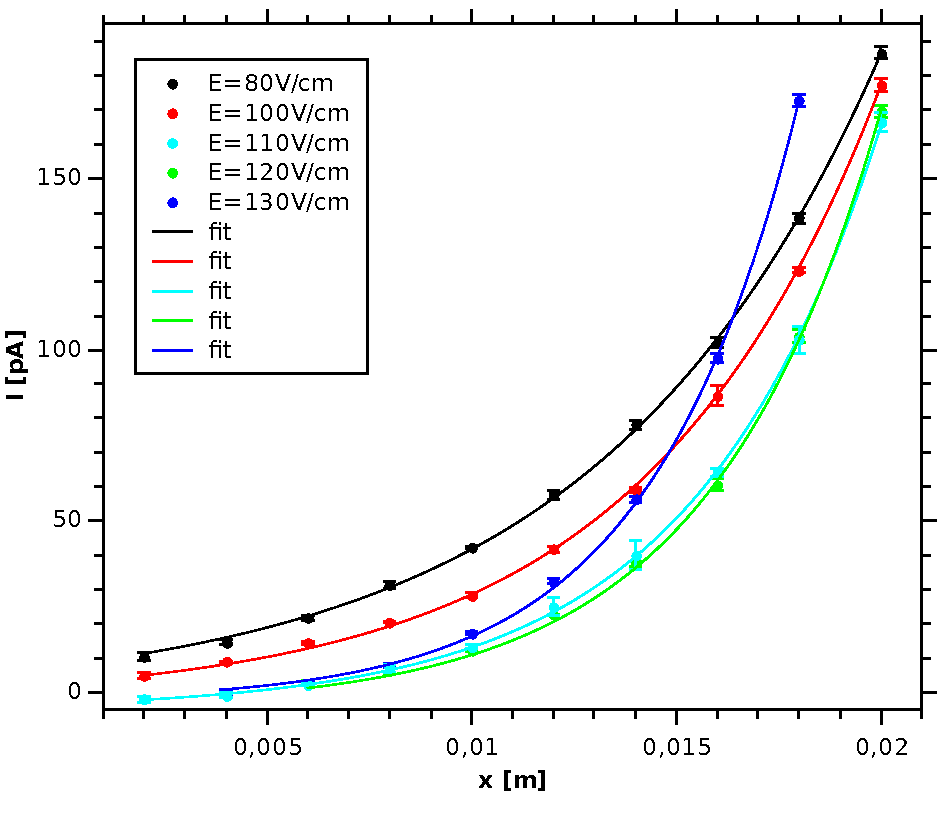
\includegraphics[width=12cm]{Graph1.pdf}
\caption{Závislost proudu na vzdálenosti elektrod pro různé intenzity elektrického pole}
\end{center}
\label{i=fx}
\end{figure}

\begin{figure}[htbp]
\begin{center}
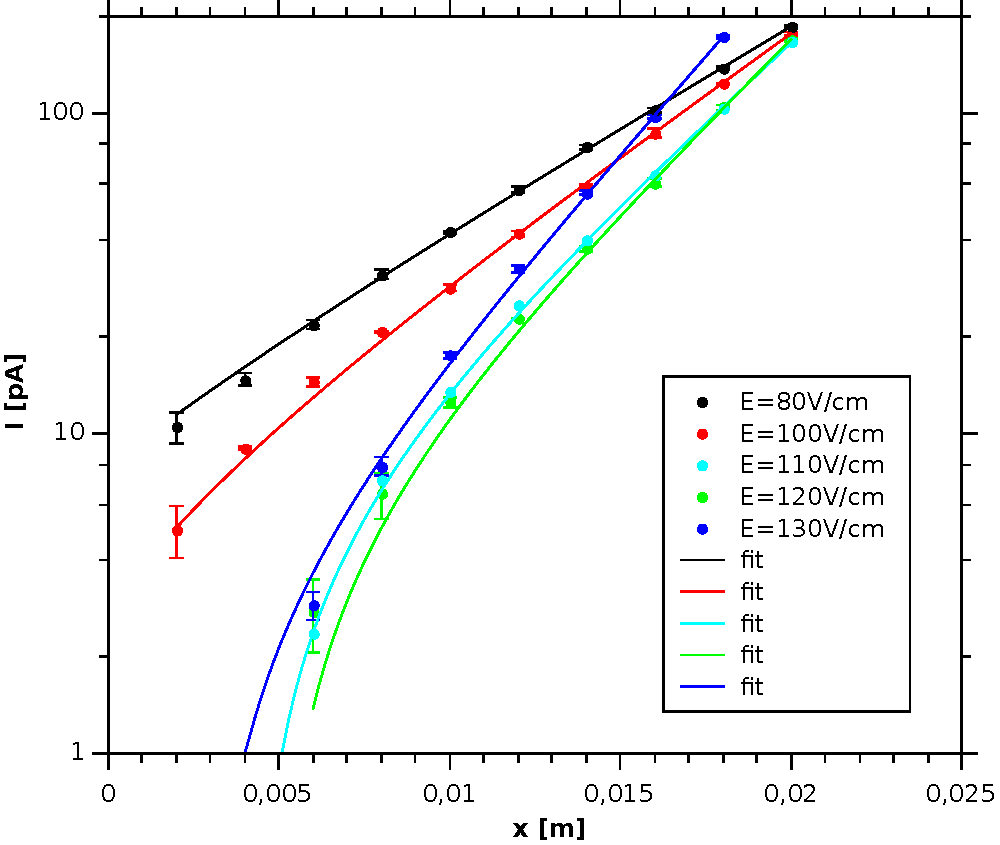
\includegraphics[width=12cm]{log.pdf}
\caption{Závislost proudu na vzdálenosti elektrod pro různé intenzity elektrického pole v logaritmické škále}
\end{center}
\label{lni=fx}
\end{figure}

V průběhu měření se ukázalo, že ampérmetr má posunutou nulu, při fitování jsem proto používal pozměněný vzorec $I = I_0 \mathrm{e}^{\alpha x} + I_\mathrm{p}$, kde $I_\mathrm{p}$ je posunutí nuly na ampérmetru. Hodnoty získané fitováním shrnuje tabulka \ref{vysl}.

\begin{table}[htbp]
\begin{center}
\begin{tabular}{|c|c|c|c|c|c|c|c|c|c|c|}
\hline
$E$[V/cm] & $\alpha$[m$^{-1}$] & $\sigma_\alpha$[m$^{-1}$] & $I_0$[pA] & $\sigma_{I_0}$[pA] & $I_\mathrm{p}$[pA] & $\sigma_{I_\mathrm{p}}$[pA] & $\frac{\alpha}{p}$[Pa$^{-1}$m$^{-1}$] & $\sigma_\frac{\alpha}{p}$[Pa$^{-1}$m$^{-1}$] \\ \hline
80 & 103,9 & 6,4 & 14,50 & 0,27 & -2,45 & 1,73 & 1,675 & 0,193 \\ \hline
100 & 174,7 & 0,7 & 5,46 & 0,09 & -2,68 & 0,48 & 2,817 & 0,273 \\ \hline
110 & 222,8 & 2,4 & 1,98 & 0,09 & -5,15 & 0,26 & 3,593 & 0,350 \\ \hline
120 & 241,8 & 6,7 & 1,38 & 0,20 & -4,52 & 2,71 & 3,899 & 0,393 \\ \hline
130 & 277,3 & 3,9 & 1,19 & 0,09 & -2,63 & 1,19 & 4,472 & 0,437 \\ \hline
\end{tabular}
\caption{Výsledky}
\label{vysl}
\end{center}
\end{table}

Tlakoměr po celou dobu ukazoval hodnotu 70\,Pa, po přepočtení na tlak v argonu je to 62\,Pa, jeho směrodatnou odchylku jsem odhadl na 10\,\%. Tato vysoká hodnota je způsobena nedostatečným ocejchováním ručičky manometru, kde je navíc logaritmická škála, takže se konkrétní hodnoty odhadovaly velmi těžko. K dalšímu zvětšení chyby došlo při přepočtu na tlak v argonu.

\begin{figure}[!htbp]
\begin{center}
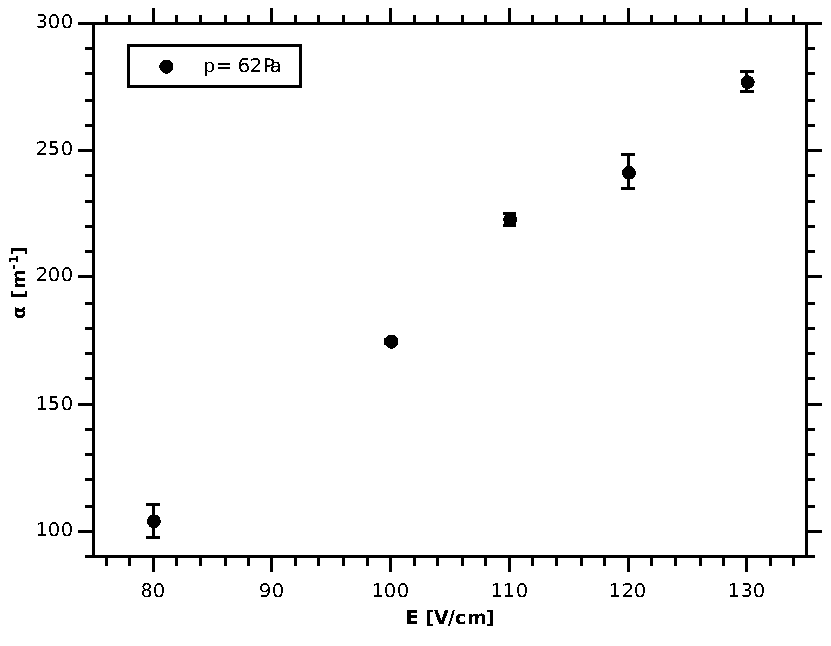
\includegraphics[width=13cm]{Graph3.pdf}
\caption{Závislost prvního Townsendova koeficientu na intenzitě elektrického pole při konstantním tlaku}
\label{obrvysledky}
\end{center}
\end{figure}

\begin{figure}[!htbp]
\begin{center}
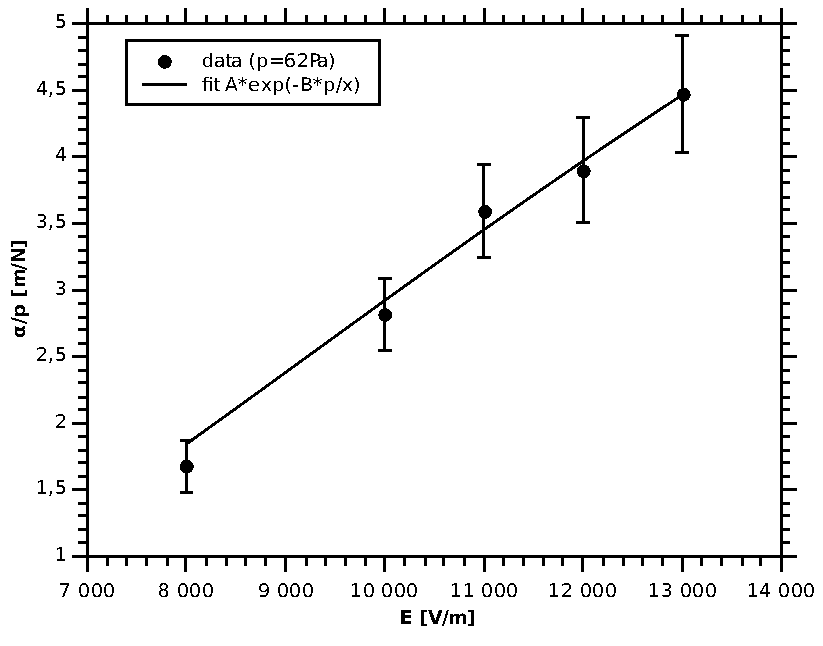
\includegraphics[width=13cm]{Graph2.pdf}
\caption{Závislost poměru $\alpha/p$ na intenzitě elektrického pole}
\label{AB}
\end{center}
\end{figure}


Fitování koeficientů A a B je na obrázku \ref{AB}. Jejich znalost můžeme využít k určení prvního ionizačního potenciálu $U_\mathrm{i}$\\
\begin{center}
$A = (18,3 \pm 2,6)\,\mathrm{m/N}$\\
$B = (306 \pm 29)\,\mathrm{Vm/N}$\\
$U_\mathrm{i} = B/A = (16,7 \pm 2,9)\,\mathrm{V}$
\end{center}


\section{Závěr}
Měření proběhlo úspěšně. Podařilo se určit Townsendův koeficient pro pět různých intenzit el. pole a tvar fitované funkce dobře souhlasí s experimentálními hodnotami. Ukázalo se, že první Townsendův koeficient roste s intenzitou elektrického pole přibližně lineárně. Také se úspěšně podařilo určit koeficienty $A$ a $B$. Vypočítaný první ionizační potenciál velmi dobře souhlasí s~tabulkovou hodnotou (15,8\,V). Slabým článkem celého měření je dle mého názoru určování tlaku, jelikož jeho chyba je v porovnání s ostatními velmi velká.
\end{document}
